\documentclass[a4paper,11pt]{article}
\usepackage[T1]{fontenc}
\usepackage{import}
\usepackage[utf8]{inputenc}
\usepackage[spanish]{babel}
\usepackage[left=1.5cm,right=1.5cm,top=1.4cm,bottom=1.5cm]{geometry}
\usepackage{graphicx}
\newcommand{\mrm}{\mathrm}
\usepackage{amsmath}
\usepackage{amsfonts}
\usepackage{xcolor}
\usepackage{tcolorbox}
\usepackage{amssymb}
\usepackage{here}
\begin{document}
\tcbset{colframe=black!50!gray,colback=gray!20,colupper=black,fonttitle=\bfseries,nobeforeafter,center title}
\setcounter{page}{1}
\pagenumbering{Roman}

\tableofcontents
\newpage
\listoffigures
\addcontentsline{toc}{section}{Índice de Figuras}
\newpage
\renewcommand{\abstractname}{Introducción}
\addcontentsline{toc}{section}{Introducción}
\vspace*{\fill}
\begin{abstract}
    Las máquinas asíncronas se utilizan en aplicaciones de hasta el rango de los MW. Su construcción sencilla con rotor tipo jaula de ardillas las convierte en motores de uso más frecuente. Estos motores asíncronos trifásicos industriales pueden ser:
    \begin{itemize}
        \item Motores trifásicos con rotor jaula de ardilla (una jaula, doble jaula, jaula tratada y ranura profunda).
        \item Motores trifásicos con polos conmutables con bobinado Dahlander.
        \item Motores trifásicos con polos conmutables con dos bobinados separados. 
    \end{itemize}
    Los motores se utilizan en los sectores industriales más variados, como por ejemplo las industrias alimentaria, química, metalúrgica, papelera, minera o las instalaciones de tratamiento de aguas. Las aplicaciones incluyen máquinas con piezas móviles a velocidad fija o variable, como por ejemplo los sistemas de elevación, como ascensores o montacargas; de transporte, como las cintas transportadoras; los sistemas de ventilación y climatización, como las unidades de tratamiento de aire; y su uso más común: las bombas y compresores.
    
    Estos hechos evidencian por qué el motor asíncrono trifásico puede considerarse como la máquina eléctrica más ampliamente utilizada en el entorno industrial.
\end{abstract}
\vspace*{\fill}
\newpage

\pagenumbering{arabic}
\setcounter{page}{1}  %%% empezamos en página 1
\section{Objetivos}
Los objetivos del presente laboratorio son:
\begin{enumerate}
    \item Hacer conocer la constitución electromecánica de los motores asíncronos.
    \item Familiarizarse con la simbología y conexionado de las máquinas eléctricas de nuestro laboratorio en los ensayos según las normas IEC y NEMA.
    \item Conexión y puesta en servicio del motor.
    \item Inversión del sentido de giro (utilizando un conmutador manual).
    \item A partir de los ensayos realizados obtener el circuito monofásico equivalente.
    \item Regirstro de los valores característicos y curvas características (FP, EF, Torque) de funcionamiento específicas de las máquinas asíncronas.
    \item Evaluación de las mediciones realizadas y registradas.
    \item Presentación del protocolo de pruebas según normas establecidas.
\end{enumerate}
\section{Precauciones}
Dados las circunstancias del laboratorio y teniendo en cuenta que los equipos son muy valiosos es que se deber tener muy en cuenta lo siguiente:
\begin{enumerate}
    \item Verificar el dimensionamiento de la instrumentación a utilizarse, así mismo constatar que los esquemas estén bien planteados.
    \item Para evitar el deterioro y/o avería de los instrumentos y equipos, \textbf{no debe accionarse los equipos bajo ningún motivo, sin la aprobación del profesor}.
    \item Para evitar el deterioro de los amperímetros, en el momento del arranque se debe poner el amperímetro de línea en corto circuito (utilizando un puente) y siempre el arranque debe hacerse en estrella-triángulo a plena tensión.
    \item Luego de unos 5 segundos hacer el cambio a triángulo y seguidamente retirar el puente del amperímetro. Si es posible hacer el arranque a tensión reducida estando el motor en la posición triángulo.
    \item La escala de todos los instrumentos debe ser la máxima.
    \item Al operar el freno, comenzar con una carga mínima y aumentarlo en forma gradual hasta llegar al máximo permisible.
\end{enumerate}
\section{Fundamento teórico}
Este motor se creó debido a la demanda de un motor síncrono polifásico con arranque propio en tamaños menores, de menos de 50 HP. Que no necesitarán excitación del campo con CD y que poseen las características de velocidad constante del motor. El rotor consiste de un devanado de jaula de ardilla embobinado o vaciado, distribuido uniformemente en las ranuras.

Cuando una corriente alterna polifásica se aplica a la armadura normal de un estator polifásico, el motor arranca como motor de inducción. Debido al rotor de polo saliente, el motor llega muy fácil a su sincronía y desarrolla con rapidez el par máximo del motor síncrono de la máquina de polos salientes.

Así el motor síncrono de inducción desarrolla el par de reluctancia, proporcional a $\sin(2\alpha)$ y al cuál se le llama a veces motor polifásico de reluctancia. Pero este es un nombre equivocado porque el motor síncrono de inducción trabaja con las características combinadas del par del motor síncrono y de inducción. Cuando está diseñado con devanados de rotor de alta resistencia, se pueden desarrollar pares de arranque bastante altos, hasta del 400\% del par a plena carga. Por otro lado, el empleo de devanados del rotor con alta resistencia ocasiona desplazamiento mayor, menor eficiencia y menor posibilidades de entrada en sincronismo con carga mediante el par de reluctancia.
\subsection{Rotor de Jaula de ardilla}
En su forma instalada, es un cilindro montado en un eje. Internamente contiene barras conductoras longitudinales de aluminio o de cobre con surcos y conectados juntos en ambos extremos poniendo en cortocircuito los anillos que forman la jaula.

El nombre se deriva de la semejanza entre esta jaula de anillos y barras y la rueda de un hámster (ruedas probablemente similares existen para las ardillas domésticas). La base del rotor se construye de un apilado de hierro de laminación.
\subsection{Funcionamiento}
Los devanados en el estator de un motor de inducción instan al campo magnético a rotar alrededor del rotor. El movimiento relativo entre este campo y la rotación del rotor induce corriente eléctrica, un flujo en las barras conductoras. Alternamente estas corrientes que fluyen longitudinalmente en los conductores reaccionan con el campo magnético del motor produciendo una fuerza que actúa tangente al rotor, dando por resultado un esfuerzo de torsión para dar vuelta al eje. En efecto, el rotor se lleva alrededor el campo magnético, pero en un índice levemente más de la rotación. La diferencia en velocidad se llama deslizamiento y aumenta con la carga.

A menudo, los conductores se inclinan levemente a lo largo de la longitud del rotor para reducir ruido y para reducir las fluctuaciones del esfuerzo de torsión que pudieron resultar, a algunas velocidades, y debido a las interacciones con las barras del estator. El número de barras en la jaula de la ardilla se determina según las corrientes inducidas en las bobinas del estator y por lo tanto según la corriente a través de ellas. Las construcciones que ofrecen menos problemas de regeneración emplean números primos de barras.

El núcleo de hierro sirve para llevar el campo magnético a través del motor. En estructura y material se diseña para reducir al mínimo las pérdidas. Las láminas finas, separadas por el aislamiento de barniz, reducen las corrientes parásitas que circulan resultantes de las corrientes de Foucault. El material, un acero bajo en carbono pero alto en silicio, con varias veces la resistencia del hierro puro, en la reductora adicional. El contenido bajo de carbono le hace un material magnético suave con pérdidas bajas por histéresis.

El mismo diseño básico se utiliza para los motores monofásicos y trifásicos sobre una amplia gama de tamaños. Los rotores para trifásica tienen variaciones en la profundidad y la forma de barras para satisfacer los requerimientos del diseño. Este motor es de gran utilidad en variadores de velocidad.
\subsection{Tipos de rotores}
Existen varios tipos de estos elementos, pero los que son más usados en la industria; es decir, los rotores para motores asíncronos de corriente alterna son 4.
\subsubsection{Rotor de jaula de ardilla simple}
Los círculos negros que se muestran en la figura representan las ranuras del rotor donde va introducido el bobinado. Existen varios tipos de ranuras, de ahí que existan varios tipos de rotores.

Este tipo de rotor es el usado para motores pequeños, en cuyo arranque la intensidad nominal supera 6 o 8 veces a la intensidad nominal del motor. Soporta mal los picos de cargas. Está siendo sustituido por los rotores de jaula de ardilla doble en motores de potencia media. Su par de arranque no supera el 140\% del nominal. 
\subsubsection{Rotor de jaula de ardilla doble}
La ranuras es doble, por este motivo tiene el nombre de ardilla doble. Las dos ranuras están separadas físicamente, aunque en el dibujo no se observe.

Este tipo de rotor tiene una intensidad de arranque de 3 o 5 veces la intensidad nominal, y su par de arranque puede ser de 230\% la nominal. Estas características hacen que este tipo de rotor sea muy interesante frente al rotor de jaula de ardilla simple. Es el más empleado en la actualidad, soporta bien las sobrecargas sin necesidad de disminuir la velocidad, lo cual le otorga mayor estabilidad.
\subsubsection{Rotor con ranura profunda}
Es una variante del rotor de jaula de ardilla simple, pero se le denomina rotor de ranura profunda. Sus características vienen a ser iguales a la del rotor de jaula simple. Es usado para motores de baja potencia que necesitan realizar continuos arranques y paradas.
\subsubsection{Rotor de anillos rozantes}
Se denominan rotores de anillo rozantes porque cada extremos del bobinado está conectado con un anillo situado en el eje del rotor. Las fases del bobinado salen al exterior por medio de unas escobillas que rozan en los anillos.

Conectando unas resistencias externas a las escobillas se consigue aumentar la resistencia rotórica, de está forma, se logra variar el par de arranque, que puede ser, dependiendo de dichas resistencias externas, del 150\% y el 250\% del par normal. La intensidad nominal no supera las 2 veces la intensidad nominal del motor.
\subsection{Aplicaciones comunes}
Los motores de la línea monofásica pueden ser clasificados como ``Motores de Uso general''; sin embargo, pueden ser empleados, sin ningún problema, en aplicaciones específicas como:
\begin{itemize}
    \item Aplicaciones en ambientes polvosos.
    \item Bombas centrífugas.
    \item Compresores.
    \item Ventiladores.
    \item Bombas de combustible.
    \item A prueba de explosión.
    \item Lavadoras y electrodomésticos en general.
\end{itemize}
\section{Equipos y máquinas eléctricas a utilizar}
\begin{enumerate}
    \item \textbf{Autotransformador variable.}
    \begin{figure}[H]
        \centering
        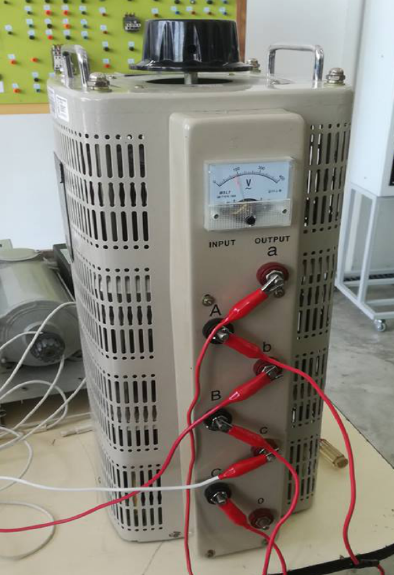
\includegraphics[scale=0.45]{autotransformador.png}
        \caption{Autotransformador variable}
    \end{figure}
    \item \textbf{Motor jaula de ardilla trifásico.}
    \begin{figure}[H]
        \centering
        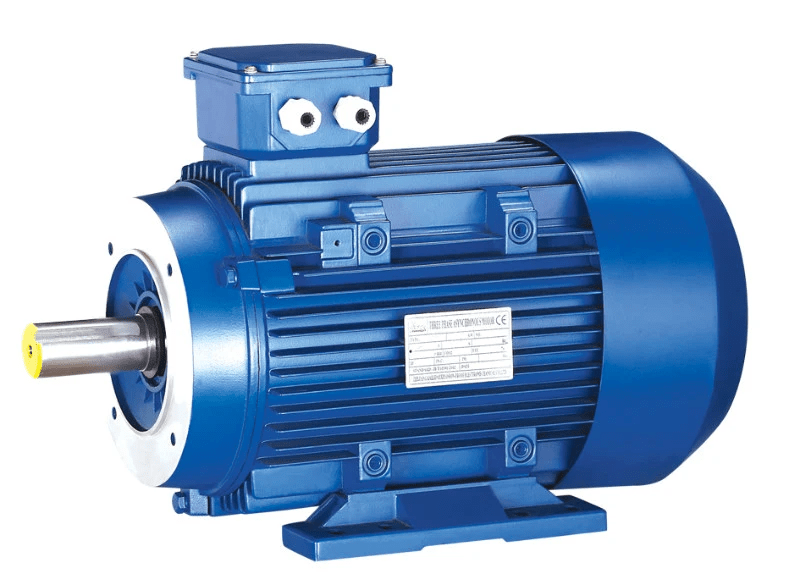
\includegraphics[scale = 0.48]{ardilla.png}
        \caption{Motor jaula de ardilla trifásico}
    \end{figure}
    \item \textbf{Banco activo de pruebas.}
    \begin{figure}[H]
        \centering
        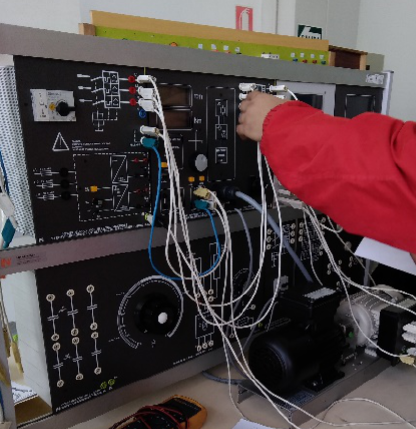
\includegraphics[scale = 0.78]{banco_activo.png}
        \caption{Banco activo de pruebas}
    \end{figure}
\end{enumerate}
\begin{table}[H]
\centering
\tcbox[left=0mm,right=0mm,top=0mm,bottom=0mm,boxsep=0mm,toptitle=0.8mm,bottomtitle=0.8mm,title=Banco activo de pruebas]{
\renewcommand{\arraystretch}{1.2}%
\begin{tabular}{c|c}
N$^{\circ}$ de pedido & SO3636-6U \\
\hline
Tensión Nominal & 230 Voltios \\
\hline
Corriente Nominal & 3 Amperios\\
\hline
Corriente Arranque & 9 Amperios\\
\hline
Torque Máximo & 10 N-m\\
\hline
Potencia Aparente & 800 VA\\
\hline
Régimen de servicio & S$_{1}$\\
\hline
RPM $\max$ & 4000\\
\hline
Grado de protección & IP$_{20}$\\
\hline
\multicolumn{2}{c}{\textbf{Amplificador Integrado}}\\
\hline
Tensión de pico & 600 Voltios\\
\hline
Tensión RMS & 400 Voltios \\
\hline
Corriente pico & 10 Amperios\\
\hline
Corriente RMS & 7 Amperios
\end{tabular}}
\hskip 1em
\tcbox[left=0mm,right=0mm,top=0mm,bottom=0mm,boxsep=0mm,toptitle=1mm,bottomtitle=1mm,title=Motor asíncrono trifásico]{
\renewcommand{\arraystretch}{1.2}%
\begin{tabular}{c|c}
N$^{\circ}$ & \\
\hline
Tensión & 400/690 Voltios \\
\hline
Corriente & 1.73/0.81 Amperios\\
\hline
Conexión & D/Y\\
\hline
Frecuencia & 60 Hz.\\
\hline
Potencia & 0.37 kW\\
\hline
Régimen de servicio & S$_{1}$\\
\hline
RPM $\max$ & 2800\\
\hline
Grado de protección & IP$_{54}$\\
\hline
IKL & B\\
\hline
Norma & VDE 0530 \\
\hline
Termostato & 120$^{\circ}$ C\\
\hline
Factor de potencia & 0.84\\
\hline
\multicolumn{2}{c}{\textbf{Motor tipo jaula de ardilla}}
\end{tabular}}
\vskip 1em
\tcbox[left=0mm,right=0mm,top=0mm,bottom=0mm,boxsep=0mm,toptitle=0.8mm,bottomtitle=0.8mm,title=Descripción de máquinas y equipos]{
\renewcommand{\arraystretch}{1.2}%
\begin{tabular}{c|c|c}
Item & Descripción general de las máquinas y equipos & Cantidad \\
\hline
1 & Manguito de acoplamiento & 01 \\
\hline
2 & Cubierta de acoplamiento & 01\\
\hline
3 & Interruptor de 04 polos & 01\\
\hline
4 & Conmutador D-Y & 01\\
\hline
5 & Fuente de corriente alterna regulable \textbf{adecuada} & 01\\
\hline
6 & Multímetro analógico/digital, FP, KW, KVARS & 02\\
\hline
7 & Multímetro digital FLUKE & 01\\
\hline
8 & Unidad condensadora & 01\\
\hline
9 & Conectores de seguridad & 04\\
\hline
10 & Juego de cables de 4 mm$^{2}$ & 25\\
\end{tabular}}
\end{table}
\section{Ensayos normalizados}
\subsection{Conexión del motor asíncrono trifásico - jaula de ardilla normalizado (IEC 34-8)}
\subsection[Medición de la resistencia del estator normalizado IEEE 112/1978]{Medición de la resistencia del estator normalizado (IEEE 112/1978 item 4.1)}
\subsection[Medición de la resistencia de aislamiento normalizado IEEE 112/1978]{Medición de la resistencia de aislamiento normalizado (IEEE 112/1978 item 4.1)}
\begin{figure}[H]
        \centering
        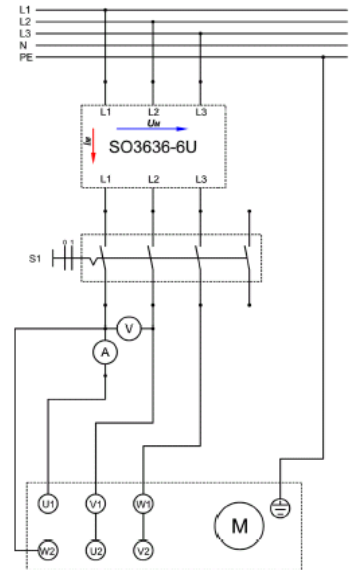
\includegraphics[scale = 1.1]{e1.png}
        \caption{Diagrama de circuito (conexión delta)}
\end{figure}
\begin{figure}[H]
        \centering
        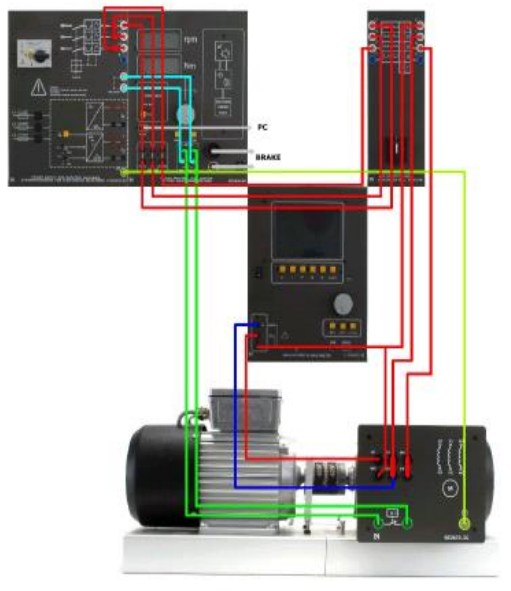
\includegraphics[scale = 0.83]{e2.png}
        \caption{Esquema de montaje (conexión delta)}
\end{figure}
\subsubsection{Circuito equivalente en un motor asíncrono}
    \begin{figure}[H]
        \centering
        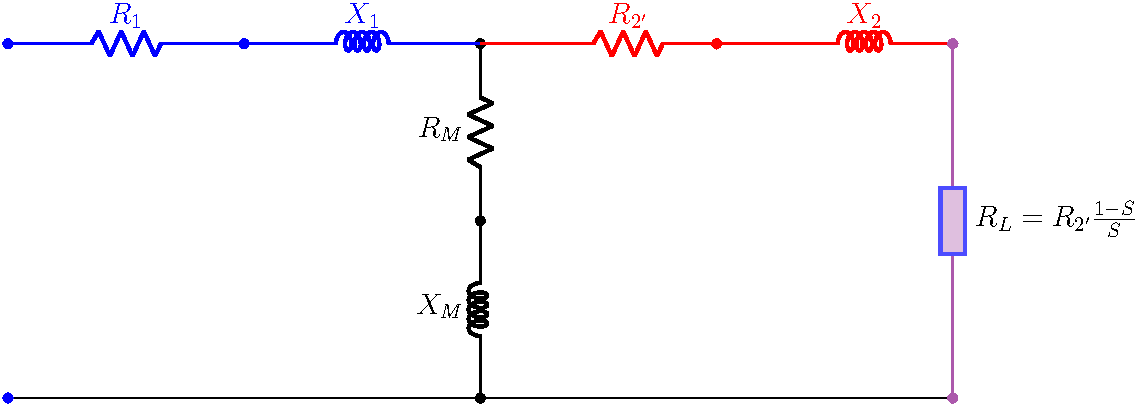
\includegraphics[scale=0.88]{d1.pdf}
        \caption{Circuito equivalente en un motor asíncrono}
    \end{figure}
\subsection[Prueba en vacío IEEE 112/1978]{Prueba en vacío (IEEE 112/1978 item 4.6)}
El montaje del motor se realiza conforme a la siguiente figura. Con el motor trifásico en vacío la tensión de alimentación se regula hasta que el voltímetro indique la tensión nominal del motor ha ser probado (ver placa). Los instrumentos de medida que se utilicen durante la práctica, ya están incluidos dentro del pupitre de prácticas.

Las condiciones son las siguientes:
\begin{itemize}
    \item La velocidad debe ser constante
    \item El eje del motor debe estar completamente libre.
    \item La frecuencia debe ser la nominal del motor.
\end{itemize}
Con la finalidad de verificar las curvas de vacío sobreponerlos con las B vs H.
\begin{align}
    B_{\max} &= \frac{V_{LL}\times 10^{-8}}{4.44\times f\, A\, N}\\
    H &= \frac{N\times \sqrt{3}\, I \, f}{L_{m}}
\end{align}
Donde:
\begin{itemize}
    \item $L_{m}$: Longitud media al paquete magnético (m).
    \item $N$: Número de vueltas del bobinado estatórico por fase.
    \item $A$: Área transversal del paquete magnético estatórico $= L\times C$
    \item $L$: Longitud del paquete magnético (m).
    \item $C$: Altura de la corona (m).
    \item $f$: Frecuencia del sistema (Hz).
    \item $V_{LL}$: Tensión de línea en Voltios.
\end{itemize}
\begin{align}
    Z_{0} &= \frac{V_{0}}{I_{0}}\\
    R_{0} &= \frac{P_{0}}{I^{2}_{0}} = R_{1} + R_{M}\\
    X_{0} &= \sqrt{Z^{2}_{0} - R^{2}_{0}} = X_{1} + X_{M}
\end{align}
\subsection[Prueba de rotor bloqueado IEEE 112/1978]{Prueba de rotor bloqueado (IEEE 112/1978 item 4.8)}
Las condiciones son las siguientes:
\begin{itemize}
    \item La corriente de línea debe ser la nominal del motor.
    \item El eje del motor debe estar trabado.
    \item La frecuencia debe ser la nominal del motor.
\end{itemize}
Para el ensayo de rotor bloqueado se utilizará exactamente el mismo esquema de conexiones que para el caso del ensayo de vacío. La única diferencia estribará en que en este caso se alimentará el motor con una tensión mucho más reducida que la nominal. A partir de 0 voltios se irá aumentando la tensión hasta que el motor alcance la corriente nominal, todo ellos manteniendo el rotor bloqueado. \textbf{Se deberá poner especial atención en no superar la corriente nominal del motor para evitar que los devanados sufran daños}. Como resultado del ensayo se registrarán la tensión, la corriente y la potencia en este ensayo.
\begin{align}
    Z_{cc} &= \frac{V_{cc}}{I_{cc}}\\[4pt]
    R_{cc} &= \frac{P_{cc}}{I^{2}_{cc}} = R_{1} + R_{2'}\\[4pt]
    X_{cc} &= \sqrt{Z^{2}_{cc} - R^{2}_{cc}} = X_{1} + X_{2'}
\end{align}
\begin{table}[H]
\centering
\tcbox[left=0mm,right=0mm,top=0mm,bottom=0mm,boxsep=0mm,toptitle=0.8mm,bottomtitle=0.8mm,title=Reactancias estatóricas y retóricas - IEEE 112 1978 ITEM 4.8]{
\renewcommand{\arraystretch}{1.2}%
\begin{tabular}{c|c|c|c|c|c}
Tipo de motor & Clase NEMA A & Clase NEMA B & Clase NEMA C & Clase NEMA D & Rotor bobinado\\
\hline
$X_{1}$ & 0.5 $X_{cc}$ & 0.4 $X_{cc}$ & 0.3 $X_{cc}$ & 0.5 $X_{cc}$ & 0.5 $X_{cc}$\\
\hline
$X_{2'}$ & 0.5 $X_{cc}$ & 0.6 $X_{cc}$ & 0.7 $X_{cc}$ & 0.5 $X_{cc}$ & 0.5 $X_{cc}$
\end{tabular}}
\end{table}
\subsection[Prueba con carga IEEE 112/1978]{Prueba con carga (IEEE 112/1978 item 4.2)}
\begin{enumerate}
\item Para la prueba con carga se tendrá que conectar el freno LN.
\item Seguir las indicaciones del profesor.
\item En forma muy atenta y delicada manipular el regulador de velocidad del freno dinámico hasta que la corriente circulante consumida por el motor es la corriente nominal.
\item Después del registro de las cargas aplicadas en el motor tomar el registro de la velocidad y el torque. Aplicando la siguiente expresión se logrará calcular la potencia útil:
\begin{align}
    P_{\mrm{util}} &= T\;(\mrm{N-m}) \times \mrm{RPM}\;(\pi /30)\\
    \mrm{EF} &= \frac{P_{\mrm{util}}}{P_{\mrm{ingreso}}}
\end{align}
\begin{table}[H]
\centering
\tcbox[left=0mm,right=0mm,top=0mm,bottom=0mm,boxsep=0mm,toptitle=0.8mm,bottomtitle=0.8mm,title=Prueba con carga (Prueba al freno)]{
\renewcommand{\arraystretch}{1.2}%
\begin{tabular}{c|c|c|c|c|c|c|c|c|c}
\multicolumn{2}{c|}{Freno} & \multicolumn{8}{c}{Motor tipo jaula de ardilla}\\
\hline
RPM & N-m & $V_{RS}$ (V) & $I_{R}$ (A) & $P_{\mrm{total}}$ (Vatios) & $Q_{\mrm{total}}$ (Vatios) & $S$ (V-A) & Eficiencia & RPM & F.P.\\
\hline
 & & & & & & & & & \\
\hline
 & & & & & & & & & \\
\hline
 & & & & & & & & &
\end{tabular}}
\end{table}
\end{enumerate}
\subsection[Ensayo de temperatura IEEE 112/1978]{Ensayo de temperatura (IEEE 112/1978 item 5.3 MET. 3)}
Consiste el registrar la temperatura y el tiempo y tener la curva Temperatura vs Tiempo. El tiempo mínimo es 4 horas cuando la temperatura comienza a disminuir en 2$^{\circ}$C durante las dos horas siguientes.
\subsection[Compensación reactiva IEC 831 y VDE 560]{Compensación reactiva IEC 831 - item 1,2 y VDE 560 item 4}
\section{Aplicaciones industriales}
Su construcción robusta e IPW adecuado hace que estos motores sean utilizados en ambientes agresivos tales como: las embarcaciones navieras, la industria textil, industrias químicas, etc. Teniendo en cuenta la categorización, sería muy importante y necesario hacer una buena selección del motor para lo cual el torque de la carga es la información base.

Las cargas más importantes son nominadas a continuación:
\begin{itemize}
    \item Compresores de aire.
    \item Electroventiladores centrífugos y axiales pequeños, medianos y grandes.
    \item Máquinas que requieren de un arranque moderado.
    \item Electrobombas centrífugas.
    \item Fajas transportadoras.
    \item Cargas que cuenten con un torque bajo, medio y elevado.
\end{itemize}
%\section{Procedimiento}
%\section{Cálculos y resultados}
\section{Cuestionario}
\begin{enumerate}
    \item \textbf{Enumere y defina las características nominales de las máquinas rotativas de inducción jaula de ardilla. Presente las características de placa del motor utilizados en su experiencia}.
    
    Son las características de funcionamiento de un motor de inducción cuando trabaja en el punto nominal y sus óptimas condiciones. Las podemos ver en la placa de características que llevan todos los motores.
    
    Las principales características de los motores de C.A. son:
    \begin{itemize}
        \item \textbf{Potencia.} Es la rapidez con la que se realiza un trabajo; en física la Potencia = Trabajo/Tiempo, la unidad del Sistema Internacional para la potencia es el Joule por segundo, y se denomina Watt (W). Sin embargo estas unidades tienen el inconveniente de ser demasiado pequeñas para propósitos industriales. Por lo tanto se utilizan el kiloWatt (kW) y el caballo de fuerza (HP).
        
        La diferencia de tensión es importante en la operación de una máquinas, ya que de esto dependerá la obtención de un mejor aprovechaiento de la operación. Los voltajes empleados más comúnmente son: 127 V, 220 V, 380 V, 440 V, 2300 V, 6000 V.
        \item \textbf{Tensiones nominales.} Son dos valores, el mayor para conectar en estrella y el menor para conectar en triángulo. Las tensiones son 400/230 V.
        \item \textbf{Velocidad nominal.} Es la velocidad de giro del rotor en el punto nominal. Es un valor alto próximo al sincronismo.
        \item \textbf{Potencia mecánica nominal.} Es la potencia que el motor entrega a la carga mecánica en forma de movimiento, cuando trabaja en el punto nominal. También se llama potencia útil, y se determina en cualquier punto de funcionamiento con la siguiente expresión:
        $$
        P_{\mrm{mec}} = \frac{2\pi}{60}MN_{r} 
        $$
        Donde:
        \begin{itemize}
            \item $P_{\mrm{mec}}$: Potencia mecánica entregada a la carga (W).
            \item $M$: Par motor (N-m).
            \item $N_{r}$: Velocidad del motor (RPM).
        \end{itemize}
        Normalmente se expresa en caballos de vapor.
        \item \textbf{Corriente.} La corriente eléctrica (I), es la rapidez del flujo de carga (Q) que pasa por un punto dado (P) en un conductor eléctrico en un tiempo (t) determinado.
        \item \textbf{Corriente nominal.} En una máquina, el valor de la corriente nominal es la cantidad de corriente que consumirá en condiciones normales de operación.
        \item \textbf{Corriente de vacío.} Es la corriente que consumirá la máquina cuando no se encuentre operando con carga y es aproximadamente del 20\% al 30\% de su corriente nominal.
        \item \textbf{Corriente de arranque.} Todos los motores eléctricos para operar consumen un excedente de corriente, mayor que su corriente nominal, que es aproximadamente de dos a ocho veces superior.
        \item \textbf{Corriente a rotor bloqueado.} Es la corriente máxima que soportará la máquina cuando su rotor esté totalmente detenido.
    \end{itemize}
    \item \textbf{¿Cómo se invierte el sentido de giro de éste motor asíncrono y cuantas posibilidades existen de hacerlo? Hagas las conexiones que se han realizado}.
    
    Se consigue permutando dos líneas cualesquiera de los tres que alimentan al motor; con ello se logra cambiar el sentido de giro del campo magnético giratorio de estator, y por ende el giro del rotor.
    
    \begin{figure}[H]
        \centering
        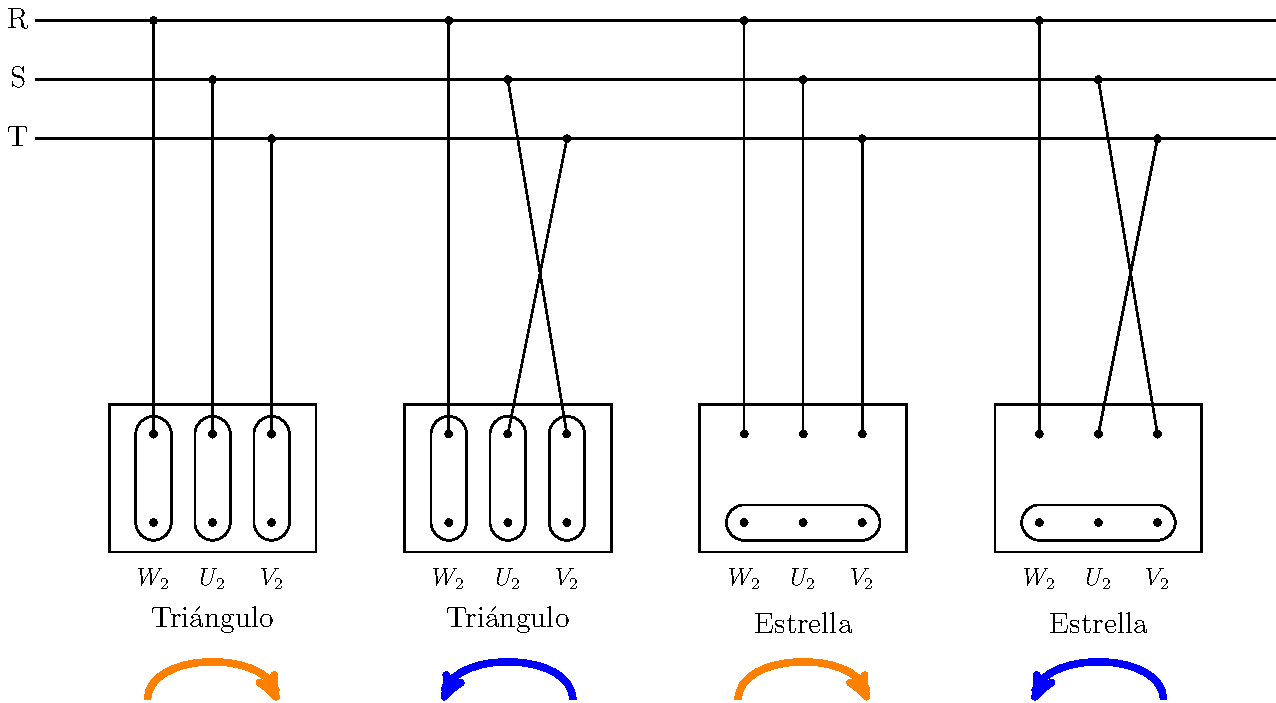
\includegraphics[scale=0.8]{P2.pdf}
        \caption{Conexiones realizadas}
    \end{figure}
    \item \textbf{Realice todos los cálculos necesarios que le conduzca a construir el diagrama equivalente monofásico valorado, referido al estator con los valores registrados y calculados en los ensayos realizados en el laboratorio}.
    
    \begin{itemize}
        \item \textbf{Prueba de vacío.}
        \begin{table}[H]
            \centering
            \tcbox[left=0mm,right=0mm,top=0mm,bottom=0mm,boxsep=0mm,toptitle=0.8mm,bottomtitle=0.8mm,title=Prueba de vacío]{
            \renewcommand{\arraystretch}{1.2}%
            \begin{tabular}{c|c|c|c|c|c}
                V (fase) & I (fase) & P (Vatios) & Torque (N-m) & fdp ($\cos\phi$) & RPM\\
                \hline
                392 & 0.22 & 30.45 & 0 & 0.35 & 3580\\
                \hline
                338 & 0.19 & 26.48 & 0 & 0.41 & 3580\\
                \hline
                300 & 0.17 & 22.26 & 0 & 0.44 & 3570\\
                \hline
                270 & 0.14 & 18.34 & 0 & 0.56 & 3550
            \end{tabular}}
            \caption{Datos obtenidos en la prueba de vacío}
        \end{table}
        \begin{align*}
            Z_{0} &= \frac{V_{0}}{I_{0}} = \frac{409.8\,\mrm{V}}{0.23} = 1781.73913\,\Omega\\
            R_{0} &= \frac{P_{0}}{I^{2}_{0}} = \frac{27\,\mrm{W}}{0.22716^{2}} = 523.25\,\Omega\\
            \cos\phi &= \frac{R_{0}}{Z_{0}} = \frac{523.25}{1781.73} = 0.293675
        \end{align*}
        Aplicando el proceso para todos los valores:
        \begin{table}[H]
            \centering
            \tcbox[left=0mm,right=0mm,top=0mm,bottom=0mm,boxsep=0mm,toptitle=0.8mm,bottomtitle=0.8mm,title=Prueba de vacío]{
            \renewcommand{\arraystretch}{1.2}%
            \begin{tabular}{c|c|c|c|c}
                Z (V/I) $\Omega$ & R ($\Omega$) & X ($\Omega$) & $\cos\phi$ calculado & $\cos\phi$ medido\\
                \hline
                1781.81818 & 629.13223 & 1667.053889 & 0.35308 & 0.35\\
                \hline
                1778.947368 & 733.518 & 1620.68 & 0.41233 & 0.41\\
                \hline
                1764.70588 & 770.24221 & 1587.7386 & 0.43647 & 0.44\\
                \hline
                1928.571428 & 935.714286 & 1686.36488 & 0.4851852 & 0.56
            \end{tabular}}
            \caption{Datos calculados de la prueba de vacío}
        \end{table}
        \item \textbf{Prueba de cortocircuito.}
        \begin{table}[H]
            \centering
            \tcbox[left=0mm,right=0mm,top=0mm,bottom=0mm,boxsep=0mm,toptitle=0.8mm,bottomtitle=0.8mm,title=Prueba de cortocircuito]{
            \renewcommand{\arraystretch}{1.2}%
            \begin{tabular}{c|c|c|c}
                V (fase) & I (fase) & P (Vatios) & fdp ($\cos\phi$)\\
                \hline
                60.4 & 0.34 & 15.22 & 0.729\\
                \hline
                99.1 & 0.55 & 40.17 & 0.73\\
                \hline
                143.7 & 0.81 & 85.9 & 0.749\\
                \hline
                175.7 & 0.99 & 130 & 0.745
            \end{tabular}}
            \caption{Datos de la prueba de cortocircuito}
        \end{table}
        \item \textbf{Prueba de carga}
        \begin{table}[H]
            \centering
            \tcbox[left=0mm,right=0mm,top=0mm,bottom=0mm,boxsep=0mm,toptitle=0.8mm,bottomtitle=0.8mm,title=Prueba de carga]{
            \renewcommand{\arraystretch}{1.2}%
            \begin{tabular}{c|c|c|c|c|c}
                V (fase) & I (fase) & P (Vatios) & Torque (N-m) & fdp ($\cos\phi$) & RPM\\
                \hline
                391 & 0.24 & 50.8 & 0.43 & 0.54 & 3560\\
                \hline
                390.7 & 0.32 & 98.4 & 0.79 & 0.784 & 3490\\
                \hline
                387.4 & 0.47 & 160.5 & 1.23 & 0.885 & 3410\\
                \hline
                388 & 0.53 & 184.5 & 1.38 & 0.9 & 3370\\
                \hline
                386 & 0.64 & 225.4 & 1.63 & 0.92 & 3300\\
                \hline
                383.8 & 0.79 & 281.12 & 1.94 & 0.927 & 3190\\
                \hline
                385.3 & 0.86 & 306.66 & 2.07 & 0.93 & 3120\\
                \hline
                380.6 & 1.02 & 350.00 & 2.15 & 0.91 & 2980
            \end{tabular}}
            \caption{Datos de la prueba de carga}
        \end{table}
    \end{itemize}
    \newpage
    \item \textbf{Grafique las curvas de vacío y corto circuito de la máquina de prueba}.
    \begin{figure}[H]
        \centering
        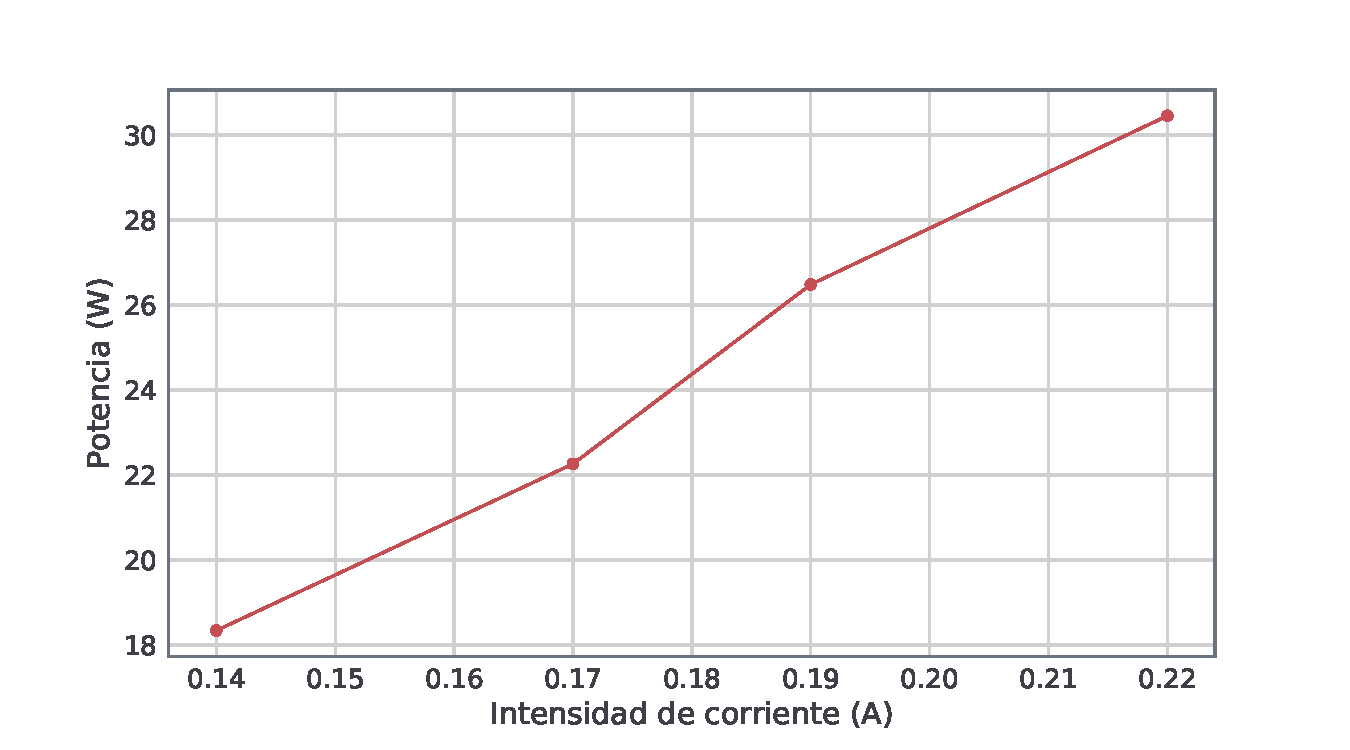
\includegraphics[scale = 0.85]{vacio1.pdf}
        \caption{Ensayo de vacío - P vs I}
    \end{figure}
    \begin{figure}[H]
        \centering
        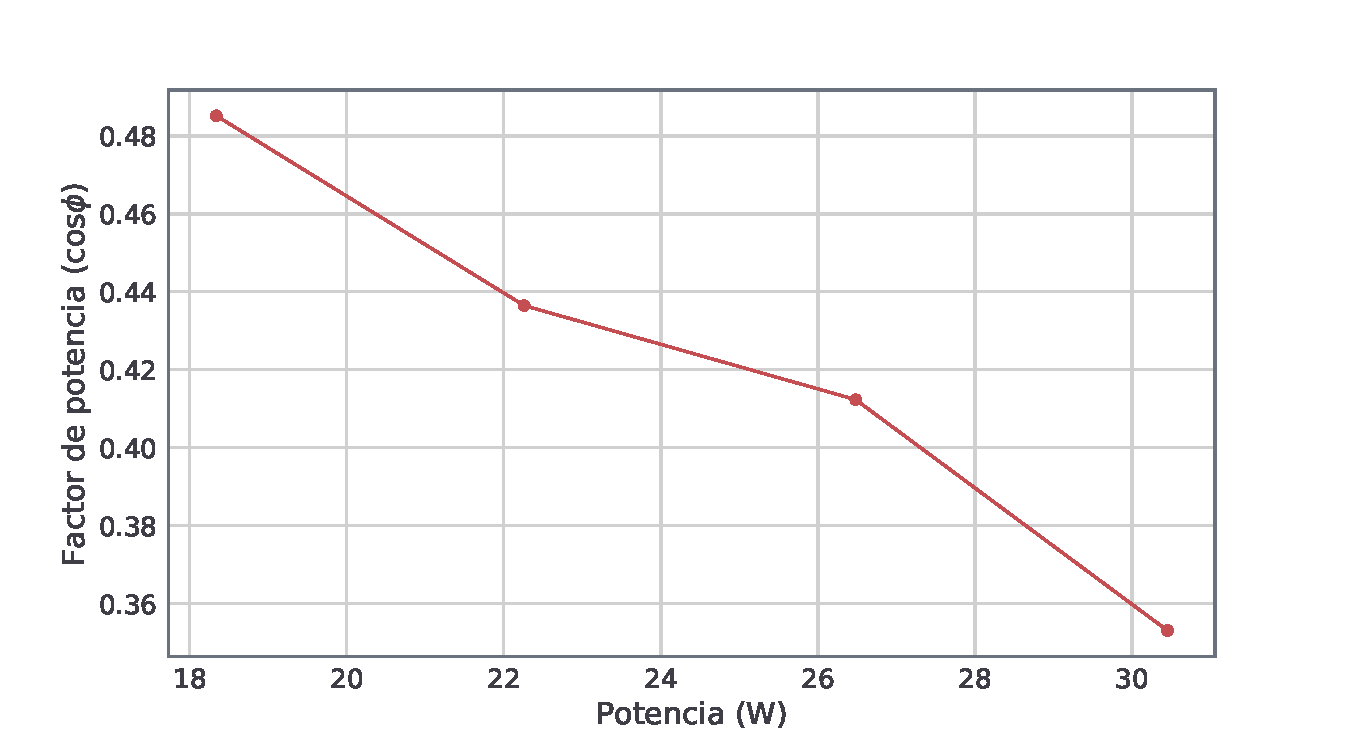
\includegraphics[scale = 0.85]{vacio2.pdf}
        \caption{Ensayo de vacío - fdp vs P}
    \end{figure}
    \begin{figure}[H]
        \centering
        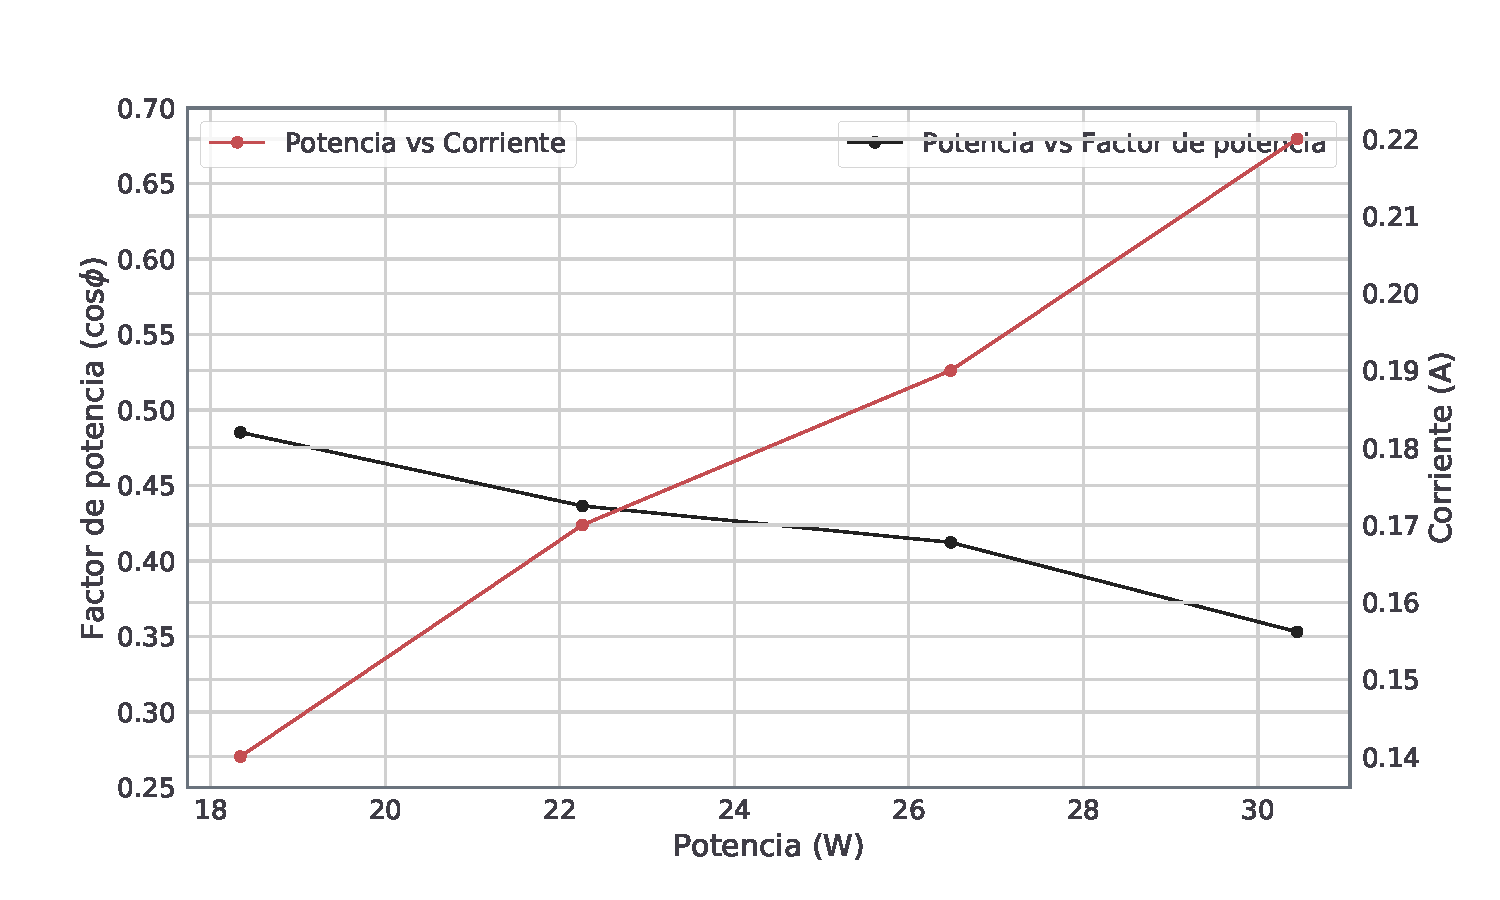
\includegraphics[scale = 0.74]{vacio3.pdf}
        \caption{Ensayo de vacío}
    \end{figure}
    \begin{figure}[H]
        \centering
        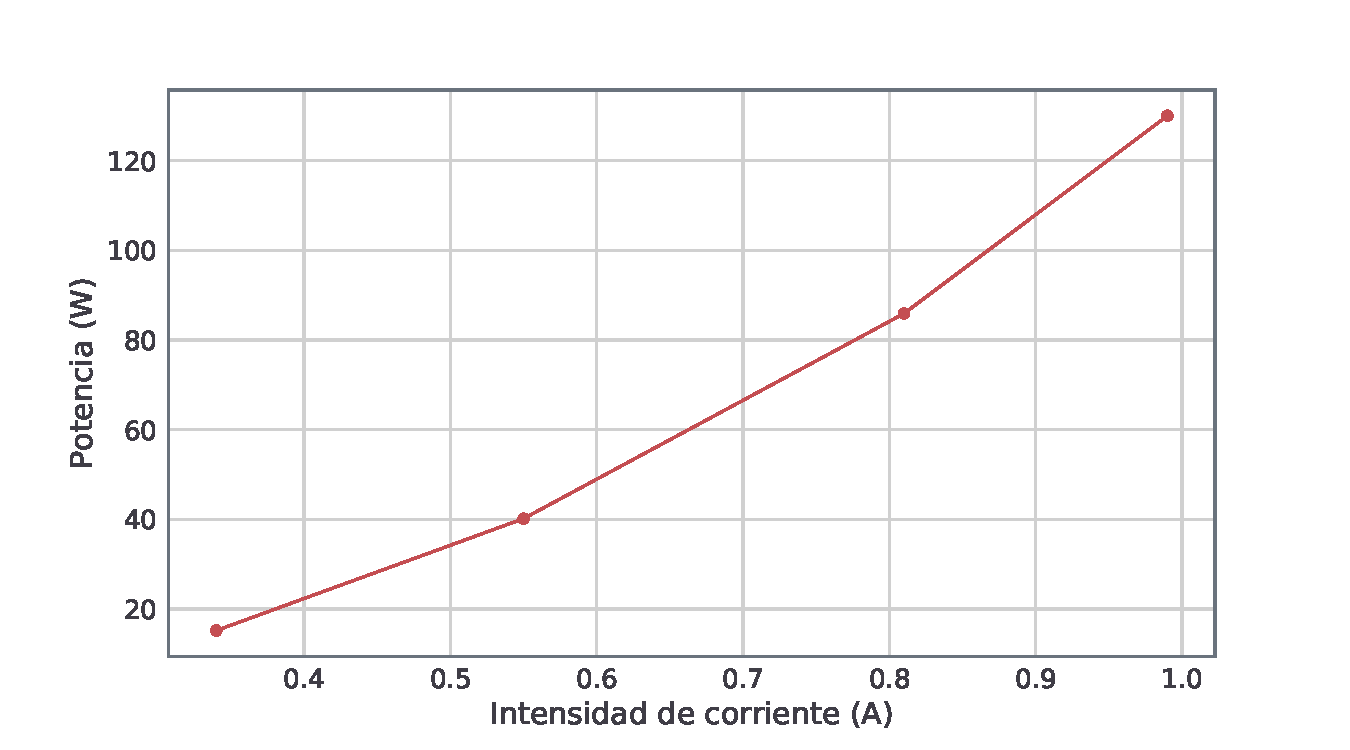
\includegraphics[scale = 0.83]{corto1.pdf}
        \caption{Ensayo de cortocircuito - P vs I}
    \end{figure}
    \begin{figure}[H]
        \centering
        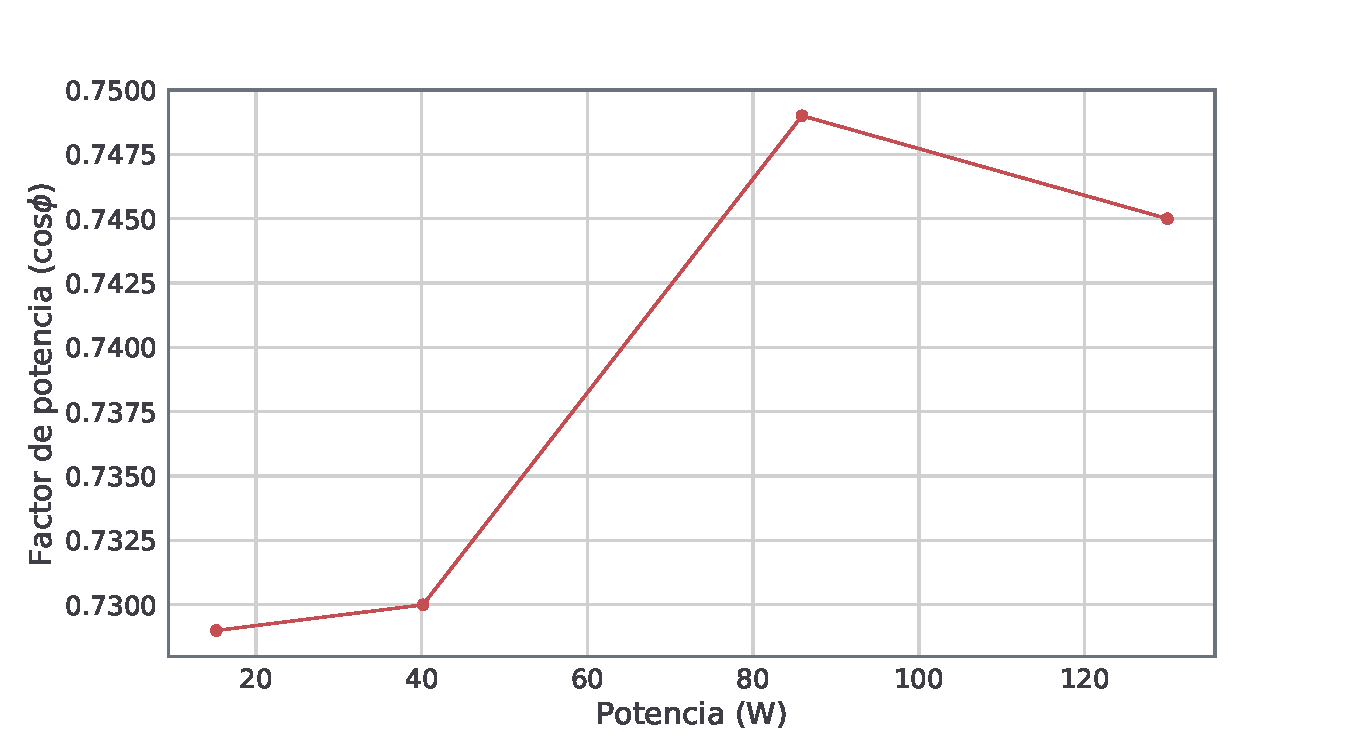
\includegraphics[scale = 0.83]{corto2.pdf}
        \caption{Ensayo de cortocircuito - fdp vs P}
    \end{figure}
    \begin{figure}[H]
        \centering
        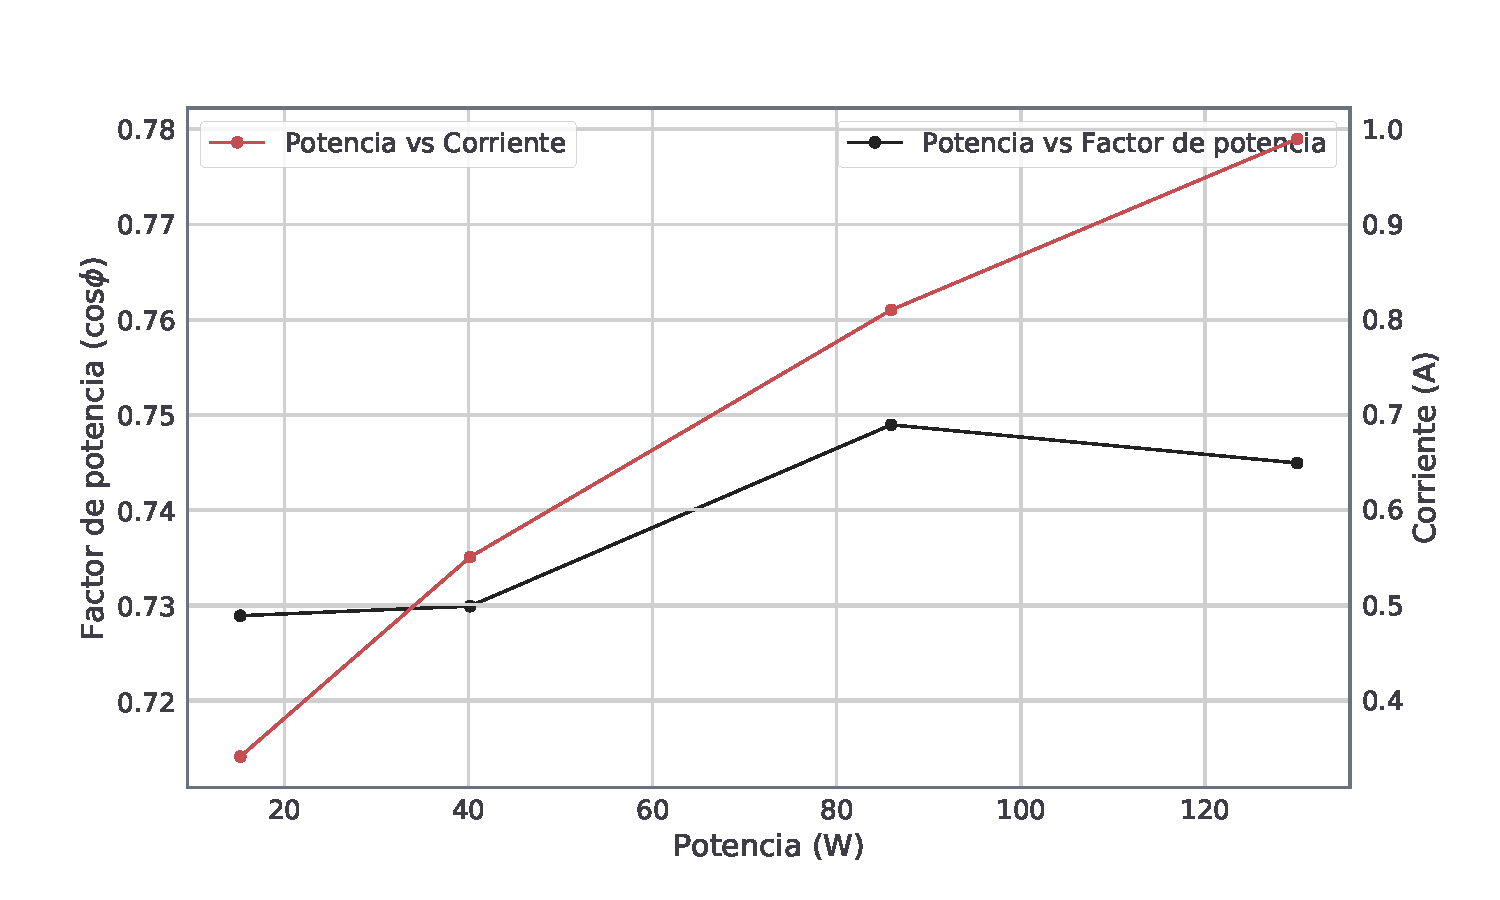
\includegraphics[scale = 0.75]{corto3.pdf}
        \caption{Ensayo de cortocircuito}
    \end{figure}
    \newpage
    \item \textbf{Grafique las curvas $P_{\mrm{nucleo}}$ vs $I_{1}$, $T$, EF, FP vs velocidad}.
    \begin{figure}[H]
        \centering
        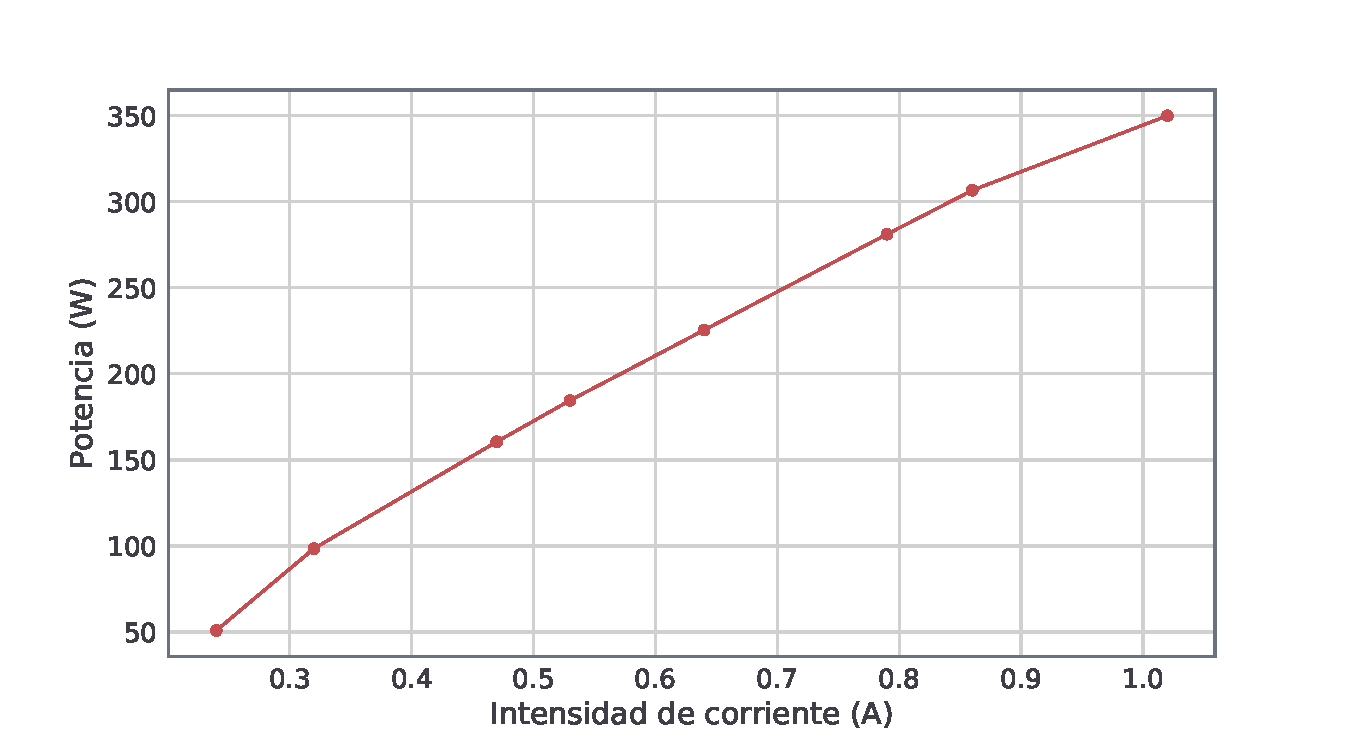
\includegraphics[scale = 0.83]{carga1.pdf}
        \caption{Ensayo de carga - P vs I}
    \end{figure}
    \begin{figure}[H]
        \centering
        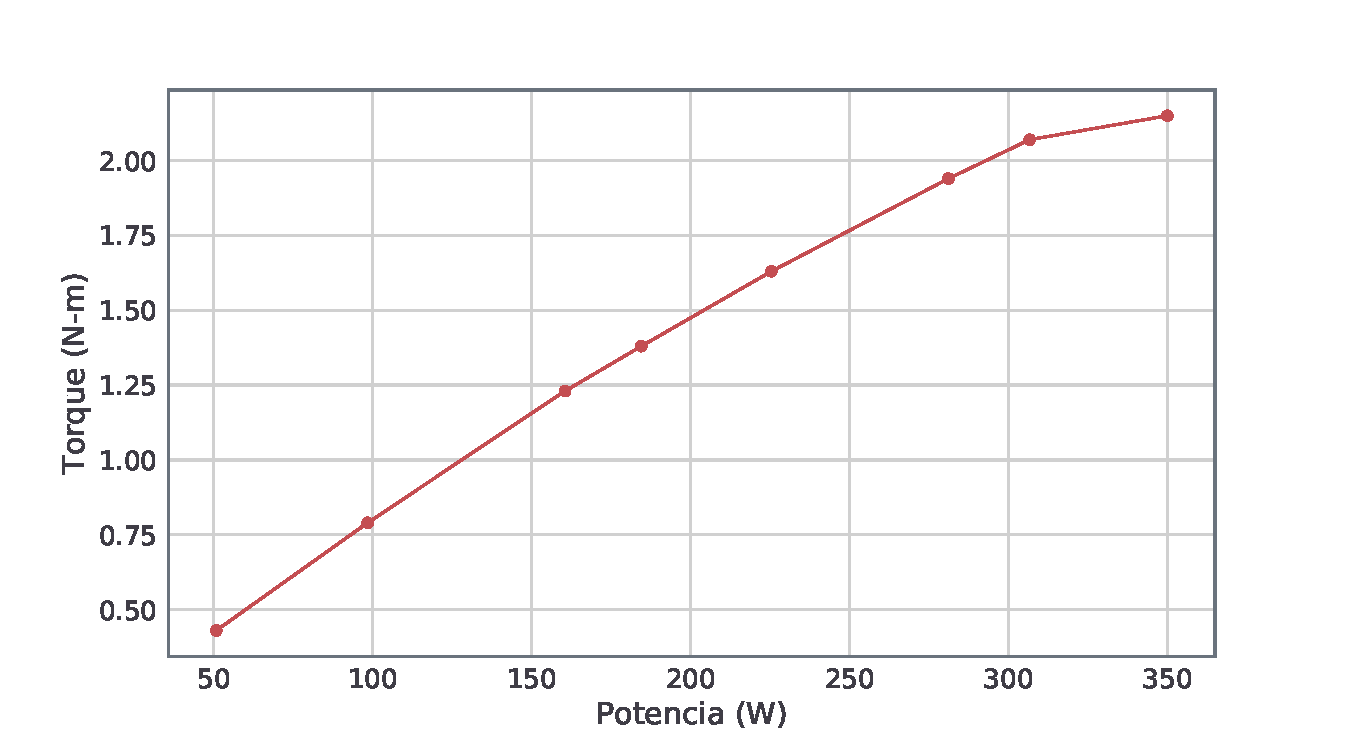
\includegraphics[scale = 0.83]{carga2.pdf}
        \caption{Ensayo de carga - T vs P}
    \end{figure}
    \begin{figure}[H]
        \centering
        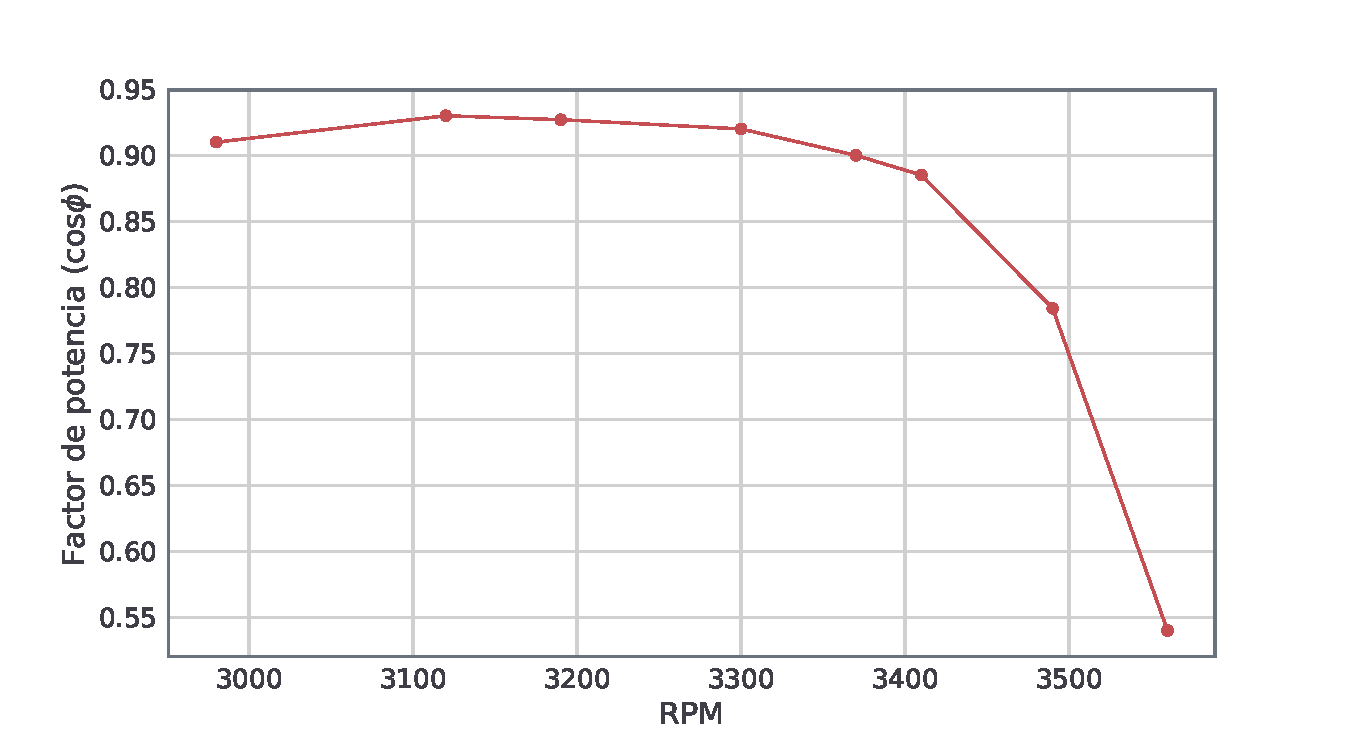
\includegraphics[scale = 0.83]{carga3.pdf}
        \caption{Ensayo de carga - fdp vs RPM}
    \end{figure}
    \begin{figure}[H]
        \centering
        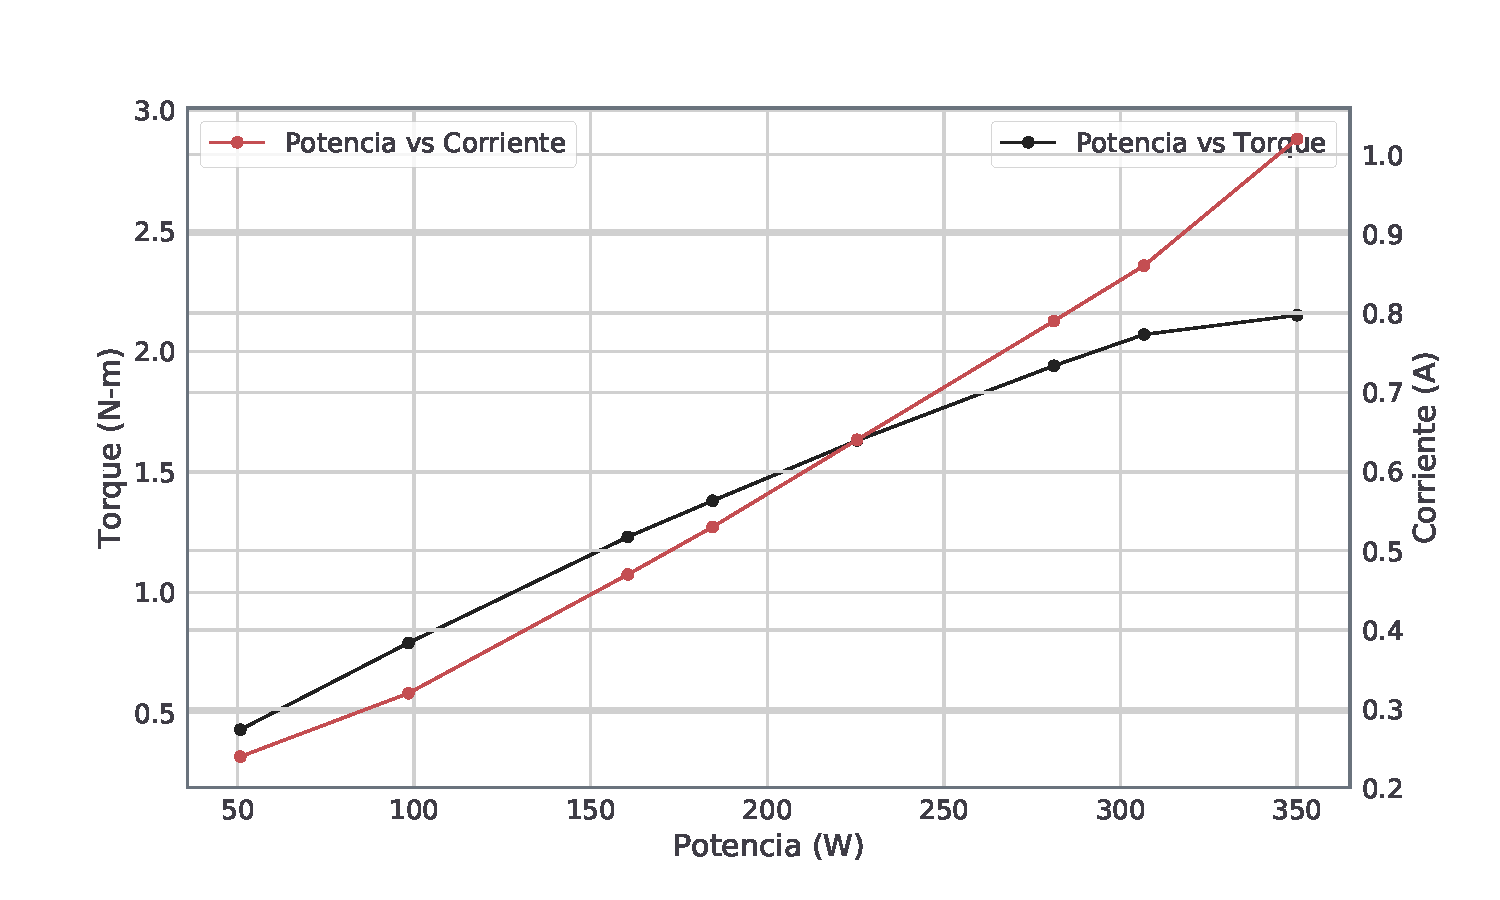
\includegraphics[scale = 0.75]{carga4.pdf}
        \caption{Ensayo de cortocircuito}
    \end{figure}
    \newpage
    \item \textbf{Determinar las pérdidas rotacionales del motor probado}.
    
    Se sabe que:
    \begin{align*}
        P_{\mrm{desarrollada}} &= 3\frac{V_{1}I\times \mrm{fdp}\times \mrm{EF}}{1000} \\
        P_{\mrm{desarrollada}} &= P_{\mrm{util}} + P_{\mrm{m}}\\
        P_{\mrm{rotacional}} &= P_{\mrm{fe}} + P_{\mrm{mec}}
    \end{align*}
    \begin{table}[H]
        \centering
        \tcbox[left=0mm,right=0mm,top=0mm,bottom=0mm,boxsep=0mm,toptitle=0.8mm,bottomtitle=0.8mm,title=$P_{\mrm{mec}}$]{
        \renewcommand{\arraystretch}{1.2}%
        \begin{tabular}{c|c|c|c|c|c|c|c|c}
            Torque (N-m) & RPM & $V_{1}$ (V) & I (A) & FDP & EF (\%) & $P_{\mrm{desarr}}$ (W) & $P_{\mrm{util}}$ (W) & $P_{\mrm{mec}}$ (W)\\
            \hline
            0.46 & 1150 & 267 & 1.29 & 0.808 & 86.43 & 72.1602 & 55.3967 & 16.7635\\
            \hline
            0.42 & 1160 & 267.7 & 1.24 & 0.814 & 83.09 & 67.3541 & 51.0194 & 16.3347\\
            \hline
            0.34 & 1190 & 267.8 & 1.17 & 0.807 & 77.45 & 58.7506 & 42.3696 & 16.3810\\
            \hline
            0.33 & 1200 & 268.8 & 1.15 & 0.808 & 73.96 & 55.4187 & 41.4690 & 13.9497
        \end{tabular}}
        \caption{Datos calculados para $P_{\mrm{mec}}$}
    \end{table}
    \begin{table}[H]
        \centering
        \tcbox[left=0mm,right=0mm,top=0mm,bottom=0mm,boxsep=0mm,toptitle=0.8mm,bottomtitle=0.8mm,title=Pérdidas rotacionales ($P_{\mrm{rotacional}}$)]{
        \renewcommand{\arraystretch}{1.2}%
        \begin{tabular}{c|c|c|c}
            $I_{\mrm{fase}}$ (A) & $P_{\mrm{fe}}$ (W) & $P_{\mrm{mec}}$ (W) & $P_{\mrm{rotacional}}$ (W)\\
            \hline
            1.29 & 706.2978 & 16.7635 & 689.5343\\
            \hline
            1.24 & 710.0061 & 16.3347 & 693.6714\\
            \hline
            1.17 & 710.5367 & 16.3810 & 694.1557\\
            \hline
            1.15 & 715.8531 & 13.9497 & 701.9034
        \end{tabular}}
        \caption{Datos calculados para $P_{\mrm{rotacional}}$}
    \end{table}
    \item \textbf{Elabore un formato de protocolo de pruebas que Ud. realizaría en las máquinas eléctricas tipo jaula de ardilla industrial}.
    \begin{figure}[H]
        \centering
        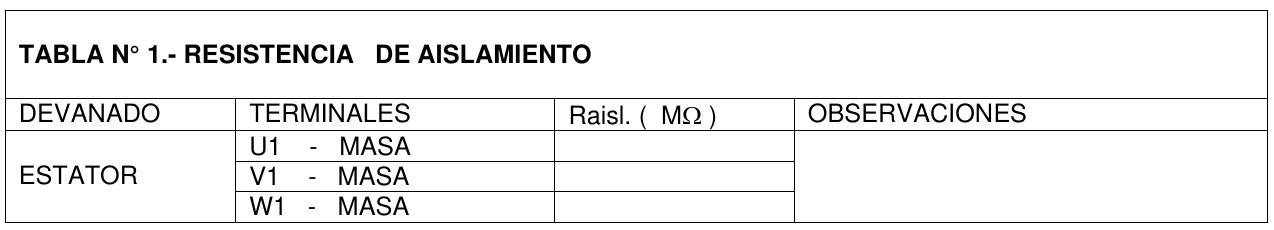
\includegraphics[scale = 0.4]{t1.png}
    \end{figure}
    \begin{figure}[H]
        \centering
        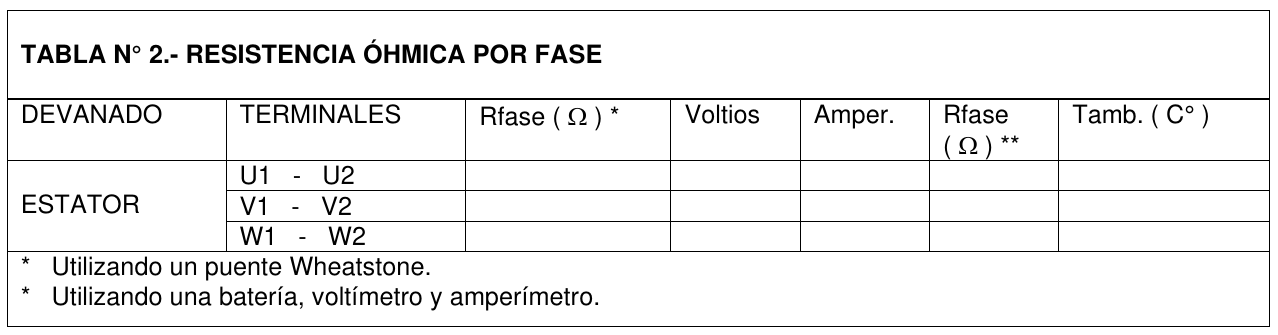
\includegraphics[scale = 0.4]{t2.png}
    \end{figure}
    \begin{figure}[H]
        \centering
        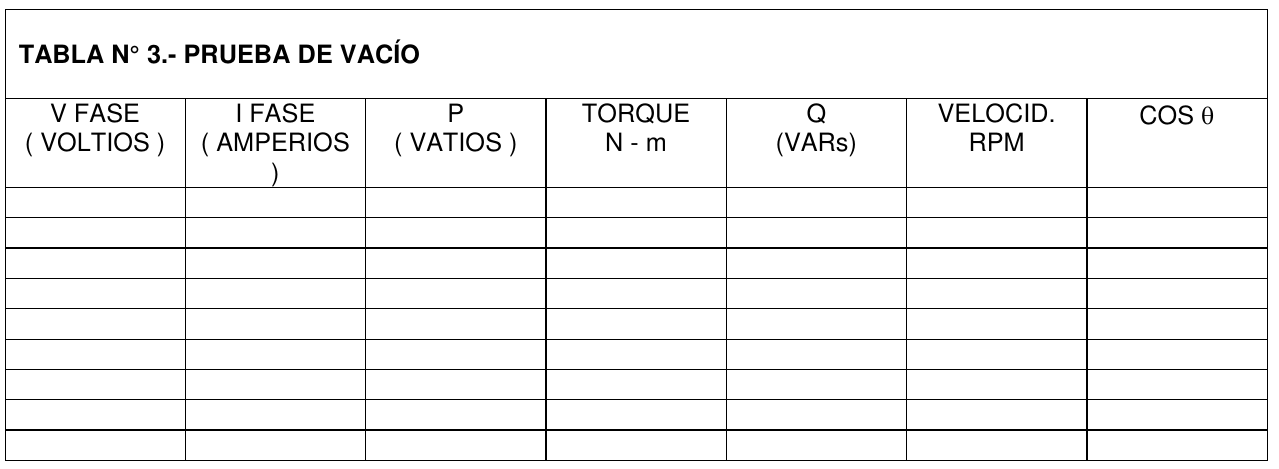
\includegraphics[scale = 0.4]{t3.png}
    \end{figure}
    \begin{figure}[H]
        \centering
        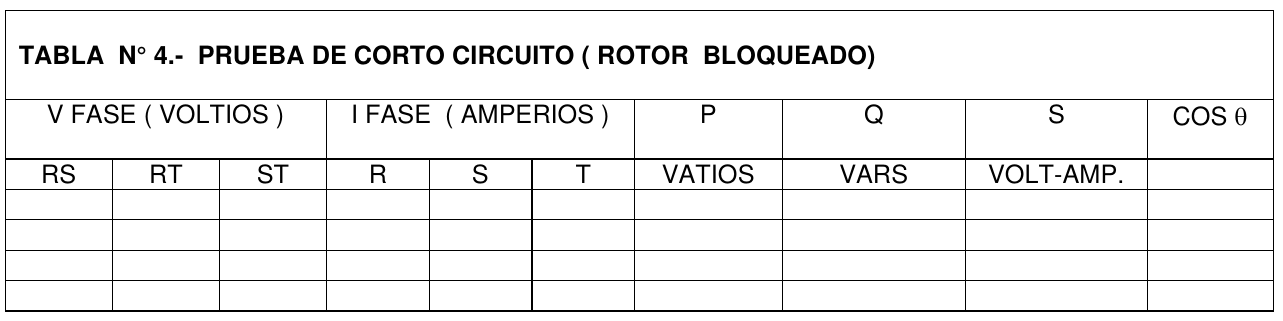
\includegraphics[scale = 0.4]{t4.png}
    \end{figure}
    \begin{figure}[H]
        \centering
        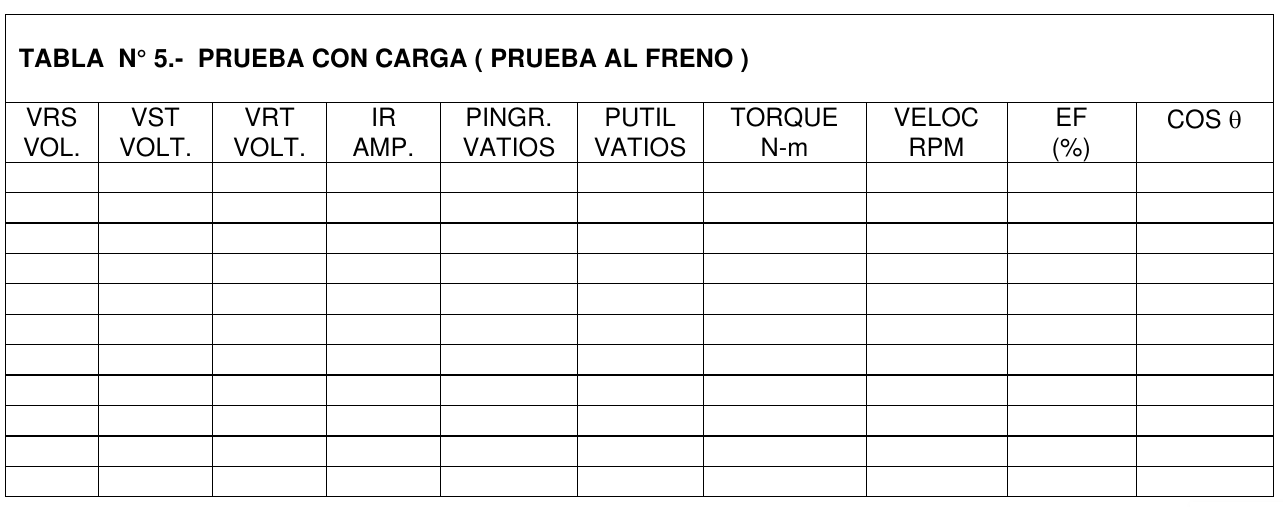
\includegraphics[scale = 0.4]{t5.png}
    \end{figure}
\end{enumerate}
\newpage
\section{Recomendaciones}
\begin{enumerate}
    \item Al regular la corriente, el cambio debe ser entre 0.1 y 0.2 A. La máquina soporta hasta 0.6 A.
    \item Se debe tener mucho cuidado y precaución en el empleo de los motores del laboratorio, para evitar el daño de los equipos y evitar accidentes.
    \item Debe revisarse que se tenga el equipo necesario, adecuado y en buen estado antes de empezar la experiencia de laboratorio.
    \item Revisar cuidadosamente que las conexiones estén bien realizadas.
    \item Si la máquinas se calienta mucho, dejar de operar por algunos minutos hasta que se enfríe hasta la temperatura ambiente.
\end{enumerate}
\section{Conclusiones}
\begin{enumerate}
    \item La impedancia del motor disminuye cuando aumentamos la corriente, dado que el voltaje disminuye, por lo tanto varía la impedancia.
    \item Conforme se aumenta la intensidad de corriente en la prueba de carga, aumenta el factor de potencia y el torque; sin embargo, la velocidad angular disminuye junto con la fuerza electromotriz.
    \item La potencia aumenta cuando la corriente incrementa.
    \item La resistencia del vacío es pequeña comparada con la reactancia.
\end{enumerate}
\newpage
\addcontentsline{toc}{section}{Anexos}
\section*{Anexos}
\begin{figure}[H]
    \centering
    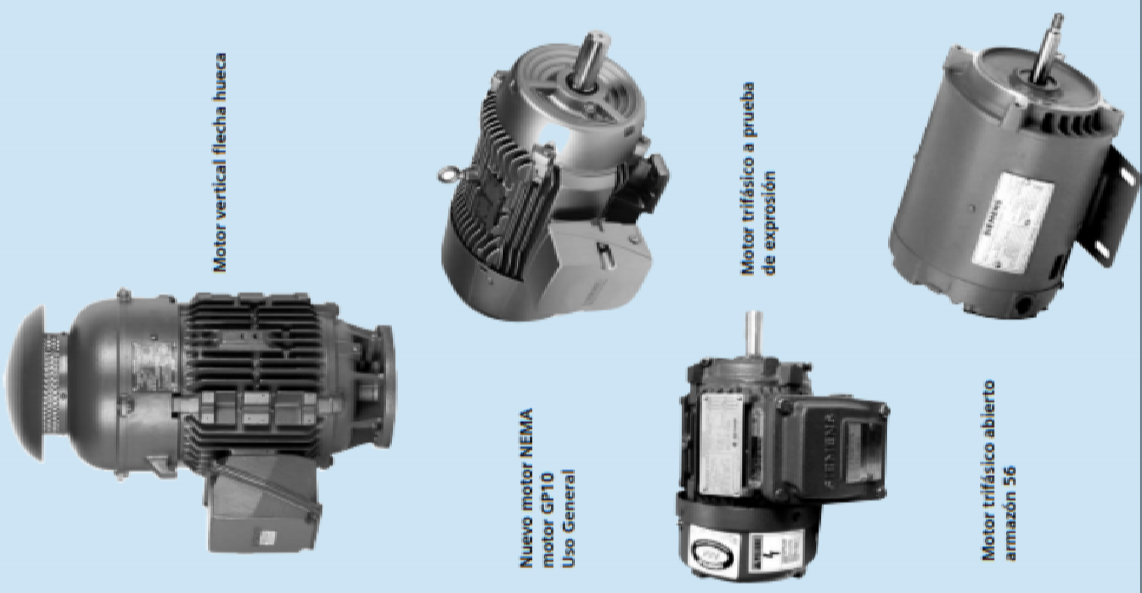
\includegraphics[scale=0.63,angle=-90]{a1.png}
\end{figure}
\newpage
\renewcommand\refname{Bibliografía}
\begin{thebibliography}{99}
\addcontentsline{toc}{section}{Bibliografía}
\bibitem{Lasheras}{Huaman L., Floren A. y Guadalupe, E. ``Guía de laboratorio de máquinas eléctricas''. {\em{Universidad Nacional de Ingeniería.}}}
\bibitem{Keyser}{Fitzgerald, A. E. y Kingsley, C. ``Teoría y análisis de las máquinas eléctricas''. {\em{Mac Graw Hill.}}}
\bibitem{Zolotorevski}{Shult, George P. ``Transformer and motors''. {\em{A division of Prentice Hall Computer 11711.}}}
\bibitem{Lasheras}{Kosow, Irving L. ``Máquinas eléctricas y transformadores''. {\em{Prentice Hall Inc 1991.}}}
\bibitem{Lasheras}{Richardson, Donald V. y Caisse, Arthur J. ``Rotating electric machinery and transformer technology''. {\em{Prentice Hall Inc 1998.}}}
\bibitem{Lasheras}{Salvador, M. G. ``Máquinas eléctricas estáticas - teoría y problemas''. {\em{Salvador Editores.}}}
\bibitem{Lasheras}{Gutiérrez, A. ``Teoría y análisis de máquinas eléctricas''.}
\bibitem{Lasheras}{Fraile M., J. ``Máquinas eléctricas''. {\em{Mac Graw Hill.}}}
\bibitem{Lasheras}{Hiziroglu, G. ``Máquinas eléctricas y transformadores''. {\em{Oxford University Press.}}}
\end{thebibliography}
\end{document}
